\documentclass{article}
\usepackage{iclr2027_conference,times}

\input{math_commands.tex}

\usepackage{hyperref}
\usepackage{url}
\usepackage{booktabs}
\usepackage{multirow}
\usepackage{amsmath}
\usepackage{amssymb}
\usepackage{bm}
\usepackage{bbm}
\usepackage{xcolor}
\usepackage{graphicx}
\usepackage{subcaption}
\usepackage{enumitem}
\usepackage{array}
\usepackage{algorithm}
\usepackage{algorithmic}
\usepackage{tikz}
\usetikzlibrary{arrows.meta,positioning,fit,backgrounds,calc}

\newcommand{\PreserveBackslash}[1]{\let\temp=\\#1\let\\=\temp}
\newcolumntype{C}[1]{>{\PreserveBackslash\centering}p{#1}}
\newcolumntype{R}[1]{>{\PreserveBackslash\raggedleft}p{#1}}

\definecolor{rowgray}{gray}{0.90}
\newcommand{\method}{\textsc{GraphPTC}\xspace}
\usepackage{xspace}

\newcommand{\best}[1]{\textbf{#1}}
\newcommand{\up}[1]{\textcolor{red!70!black}{#1}}
\newcommand{\down}[1]{\textcolor{blue!70!black}{#1}}

\title{\method: Modeling Programmatic Tool Calling as a Dynamic Execution Graph}

\author{Anonymous authors\\
Paper under double-blind review}

\begin{document}

\maketitle

\begin{abstract}
Tool calling has become the primary way large language models act on external environments, and its form is shifting from issuing one tool call per model turn toward Programmatic Tool Calling (PTC), where a model writes a program that composes many tool calls, control flow, and intermediate data processing inside a single block executed in a persistent runtime.
PTC reduces model-tool interaction rounds and expresses in-block control flow that a per-call protocol cannot, yet across program blocks its execution history remains a linear sequence of code, standard output, and errors.
This linear history leaves cross-block dependencies unrepresented, execution progress implicit, and decision feedback unstructured, so the agent repeatedly reconstructs prior results and their relations by re-reading raw text.
In this paper we introduce \method, which preserves the programmatic expressiveness of PTC and maintains a task-level dynamic execution graph from real running traces.
\method models the internal logic of each block as a typed subgraph of tool effects, artifacts, states, and failures, and models cross-block dependencies as a multi-relation graph over which the agent declares intent and chooses to continue, patch a failed step, or replan a dependency path.
Experiments on seven tool-use benchmark settings with four backbone models show that \method improves over both Direct Tool Calling and PTC on every benchmark, reaches a given accuracy with 1.5 to 3 times fewer interaction rounds than Direct Tool Calling, and widens its advantage on complex long-horizon tasks.
\end{abstract}

\section{Introduction}
\label{sec:intro}

Tool calling is the primary interface through which large language models (LLMs) act on external environments, and its form has been evolving.
Early agents issue a single tool call per model turn and read its result before deciding the next call, following the reasoning-and-acting paradigm~\citep{yao2023react,schick2023toolformer,qin2024toolllm}.
Recent systems instead adopt \emph{Programmatic Tool Calling} (PTC), where the model writes a program that composes many tool calls with loops, conditionals, and intermediate data processing, and the program runs in a persistent runtime whose variables carry across turns~\citep{gao2023pal,wang2024codeact,smolagents2025,anthropic2025ptc}.
By packing a coherent phase of work into one executable block, PTC reduces the number of model-tool interaction rounds, expresses control flow that a call-per-turn protocol cannot, and lets a later block reuse variables produced by an earlier one.
However, the expressiveness that PTC gains inside a block is not matched by how it organizes work across blocks.

Across blocks, the history that a PTC agent conditions on is a flat sequence of code, standard output, and error text ordered by time, which is a lossy record of what execution did.
A single block on the AppWorld benchmark~\citep{trivedi2024appworld} issues five to ten tool calls whose read or write effects and produced values are flattened into one output string, and a task spans more than one hundred such values across a dozen blocks.
When the agent later needs to know whether a write took effect, which earlier value a new step depends on, or whether two differently phrased queries returned the same content, it has to reconstruct these relations by re-reading raw text.
This difficulty stems from a representation that stores execution as concatenated strings and never as the dependency structure that execution induces.

\begin{figure}[t]
\centering
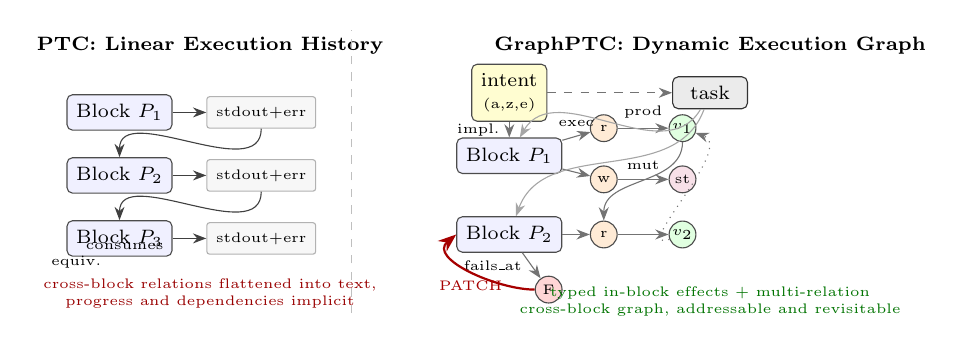
\begin{tikzpicture}[
  font=\scriptsize,
  block/.style={rounded corners=2pt, draw=black!70, fill=blue!6, minimum width=1.05cm, minimum height=0.45cm, align=center},
  gnode/.style={circle, draw=black!70, minimum size=0.34cm, inner sep=0.5pt, align=center},
  task/.style={rounded corners=2pt, draw=black!80, fill=black!8, minimum width=0.95cm, minimum height=0.4cm, align=center},
  art/.style={gnode, fill=green!12},
  call/.style={gnode, fill=orange!16},
  st/.style={gnode, fill=purple!12},
  fail/.style={gnode, fill=red!16},
  intent/.style={rounded corners=2pt, draw=black!70, fill=yellow!18, minimum width=0.9cm, minimum height=0.38cm, align=center},
  rel/.style={->, >=Stealth, draw=black!55, thin},
  seq/.style={->, >=Stealth, draw=black!75},
]

% ============ Left panel: PTC linear history ============
\node[align=center, font=\scriptsize\bfseries] at (1.7,2.55) {PTC: Linear Execution History};

\node[block] (b1) at (0.55,1.7) {Block $P_1$};
\node[block] (b2) at (0.55,0.9) {Block $P_2$};
\node[block] (b3) at (0.55,0.1) {Block $P_3$};
\node[draw=black!30, fill=black!3, rounded corners=1pt, minimum width=1.35cm, minimum height=0.4cm, align=center] (o1) at (2.35,1.7) {\tiny stdout+err};
\node[draw=black!30, fill=black!3, rounded corners=1pt, minimum width=1.35cm, minimum height=0.4cm, align=center] (o2) at (2.35,0.9) {\tiny stdout+err};
\node[draw=black!30, fill=black!3, rounded corners=1pt, minimum width=1.35cm, minimum height=0.4cm, align=center] (o3) at (2.35,0.1) {\tiny stdout+err};
\draw[seq] (b1)--(o1); \draw[seq] (b2)--(o2); \draw[seq] (b3)--(o3);
\draw[seq] (o1) to[out=-90,in=90] (b2);
\draw[seq] (o2) to[out=-90,in=90] (b3);
\node[align=center, text=red!60!black, font=\tiny] at (1.7,-0.6) {cross-block relations flattened into text,\\ progress and dependencies implicit};

% divider
\draw[black!25, dashed] (3.5,-0.85) -- (3.5,2.75);

% ============ Right panel: GraphPTC ============
\node[align=center, font=\scriptsize\bfseries] at (8.05,2.55) {\method: Dynamic Execution Graph};

\node[task] (tk) at (8.05,1.95) {task};
\node[intent] (in) at (5.5,1.95) {intent\\ \tiny (a,z,e)};

\node[block] (gb1) at (5.5,1.15) {Block $P_1$};
\node[block] (gb2) at (5.5,0.15) {Block $P_2$};

\node[call] (c1) at (6.7,1.5) {\tiny r};
\node[call] (c2) at (6.7,0.85) {\tiny w};
\node[art]  (a1) at (7.7,1.5) {\tiny $v_1$};
\node[st]   (s1) at (7.7,0.85) {\tiny st};
\node[call] (c3) at (6.7,0.15) {\tiny r};
\node[art]  (a2) at (7.7,0.15) {\tiny $v_2$};
\node[fail] (f1) at (6.0,-0.55) {\tiny F};

% intent binding
\draw[rel] (in)--(gb1) node[midway,left,font=\tiny]{impl.};
\draw[rel, dashed] (in) to[out=0,in=180] (tk);

% block1 internals
\draw[rel] (gb1)--(c1) node[midway,above,font=\tiny]{exec};
\draw[rel] (gb1)--(c2);
\draw[rel] (c1)--(a1) node[midway,above,font=\tiny]{prod};
\draw[rel] (c2)--(s1) node[midway,above,font=\tiny]{mut};

% block2 internals + cross-block
\draw[rel] (gb2)--(c3);
\draw[rel] (c3)--(a2);
\draw[rel] (a1) to[out=-90,in=90] (c3) node[midway,right,font=\tiny]{consumes};
\draw[rel, dotted] (a2) to[out=200,in=-20] (a1) node[midway,below,font=\tiny]{equiv.};
\draw[rel] (gb2)--(f1) node[midway,left,font=\tiny]{fails\_at};

% blocks belong to task
\draw[rel, black!35] (tk) to[out=-120,in=60] (gb1);
\draw[rel, black!35] (tk) to[out=-110,in=70] (gb2);

% PATCH loop back
\draw[->, >=Stealth, red!65!black, thick] (f1) to[out=180,in=-140] node[midway,below,font=\tiny,text=red!65!black]{PATCH} (gb2.west);

\node[align=center, text=green!45!black, font=\tiny] at (8.05,-0.7) {typed in-block effects + multi-relation\\ cross-block graph, addressable and revisitable};

\end{tikzpicture}
\vspace{-2mm}
\caption{PTC records execution as a linear stream of code and output where cross-block dependencies and progress are lost, whereas \method maintains a dynamic execution graph that models the internal effects of each block (tool calls with read $r$ or write $w$ effects, artifacts $v$, states st, failures F) and cross-block dependencies (consumes, equivalence, supersession), over which a declared intent selects continue, patch, replan, or answer.}
\label{fig:overview}
\vspace{-3mm}
\end{figure}


The concatenated representation produces three limitations that build on one another.
\label{sec:intro-limit}
At the representation layer, the history is a \emph{linear execution context}, where call provenance, artifact consumption, and state versioning have no unified form, so the agent rebuilds prior results and their relations from scratch.
At the analysis layer, feedback carries \emph{implicit execution progress}, because it never relates what a block intended to achieve to what it actually changed, and a block that raises no error can still re-fetch an existing result without advancing the task.
At the decision layer, standard output and errors give \emph{unstructured decision feedback} that describes only the current block, leaving the agent to infer from scattered history whether to proceed, fix the program, or change strategy, and it easily repeats a prior attempt or extends an unproductive path.

To address these limitations, we introduce \method, which keeps the programmatic expressiveness of PTC and maintains a task-level \emph{dynamic execution graph} built incrementally from real running traces.
As shown in Figure~\ref{fig:overview}, \method changes two structural aspects of PTC.
First, it models the internal logic of each block, so a code execution becomes a typed subgraph of tool calls with read or write effects, produced artifacts, state versions, and localized failures instead of an opaque output string.
Second, it models cross-block dependency as a multi-relation graph instead of a linear text stream, linking equivalent results, reused artifacts, and superseded states so that history becomes addressable.
Building on these two changes, \method runs three stages.
Graph-based execution modeling projects each trace into a shared typed graph and links cross-block dependencies.
Graph-based progress assessment binds a declared intent to the graph change it produces and separates new results from repeated ones.
Graph-based action selection turns the graph into a bounded summary over which the agent chooses to continue, patch a failed step, replan a dependency path, or answer.

We evaluate \method on seven tool-use benchmark settings with four backbone LLMs.
\method improves over both Direct Tool Calling and PTC on every benchmark, by $7.4$ points over PTC on average, and it reaches a given accuracy with $1.5$ to $3$ times fewer interaction rounds than Direct Tool Calling.
Its advantage also widens with task complexity, reaching $43$ points over Direct Tool Calling on the hardest tasks, and it transfers across closed and open backbones.
Our contributions are three-fold.
\begin{itemize}[leftmargin=1.2em, itemsep=-0.3ex, topsep=0ex]
    \item \textbf{Graph-Structured Tool Calling.} To the best of our knowledge, \method is the first framework that models programmatic tool calling as a task-level dynamic execution graph, capturing in-block tool effects and cross-block dependencies that a linear history discards.
    \item \textbf{Graph-Guided Execution.} We bind a declared intent to the graph change it produces and construct a bounded graph feedback, which lets the agent judge progress from graph effects and treat recovery as an addressable graph operation over continue, patch, replan, and answer.
    \item \textbf{Consistent Empirical Gains.} On seven settings and four backbones, \method surpasses Direct Tool Calling and PTC on the primary metric, widens its advantage on complex long-horizon tasks, and reduces interaction rounds at equal accuracy.
\end{itemize}

\section{Related Work}

\textbf{Tool Calling and Programmatic Agents.}\quad
Tool-augmented LLMs have progressed from single-call protocols to programmatic execution.
Early work teaches models to emit one structured tool call per turn and interleave it with reasoning, as in Toolformer~\citep{schick2023toolformer}, ReAct~\citep{yao2023react}, ToolLLM~\citep{qin2024toolllm}, and Gorilla~\citep{patil2023gorilla}, and multi-agent frameworks such as AutoGen~\citep{wu2023autogen} and MetaGPT~\citep{hong2024metagpt} coordinate several such agents.
A parallel line expresses actions as code, starting from program-aided reasoning~\citep{gao2023pal,chen2023pot} and maturing into code-as-action agents that emit executable programs calling tools in a live interpreter, including CodeAct~\citep{wang2024codeact}, code-agent libraries~\citep{smolagents2025}, and recent programmatic tool calling that runs a model-written program against many tools in one runtime~\citep{anthropic2025ptc}.
These programmatic approaches gain expressiveness and fewer interaction rounds inside a block, yet they still hand the model a linear transcript of code and output across blocks, and the dependency structure that execution induces is left for the model to reconstruct.

\textbf{Feedback, Reflection, and Memory for Agents.}\quad
A second line improves how agents use their own history.
Reflection methods summarize past outcomes into natural-language advice, as in Reflexion~\citep{shinn2023reflexion} and Self-Refine~\citep{madaan2023selfrefine}, but the summary is unstructured text and does not track which concrete result each step produced.
Memory systems extend the usable context, from paged memory in MemGPT~\citep{packer2024memgpt} to knowledge-graph and agentic memory stores~\citep{rasmussen2025zep,xu2025amem}, and cognitive-architecture views organize an agent around explicit state~\citep{sumers2024coala}.
These systems index facts and entities for later retrieval, whereas GraphPTC indexes what an execution did, namely the call provenance, artifact flow, state versioning, and localized failures inside and across code blocks, and turns that structure into the signal that steers the next action.

In this work, we target the execution history of programmatic tool calling, with the goal of turning a linear transcript of code and output into a structure an agent can reason over.
Unlike per-call agents that never compose tool calls into programs, and unlike programmatic agents that keep execution history as flat text, \method adopts a more deliberate design by maintaining a task-level dynamic execution graph that models in-block tool effects and cross-block dependencies, and by driving action selection from a bounded summary of that graph.

\section{\method}
\label{sec:method}

\method retains the ability of PTC to organize many tool calls and intermediate data processing into one executable program, and augments it with a task-level dynamic execution graph that is built from real running traces.
The design follows three stages that respond one to one to the three limitations of Section~\ref{sec:intro-limit}.
Graph-based execution modeling resolves the linear execution context, graph-based progress assessment resolves the implicit execution progress, and graph-based action selection resolves the unstructured decision feedback.

We first fix notation.
Let $P_t$ be the program the agent writes at round $t$, $\mathcal{G}_{t-1}$ the accumulated graph before this round, and $\tau_t$ the trace obtained by executing $P_t$ with instrumented tools.
When the agent writes $P_t$ it also declares an intent $I_t$.
The runtime projects the trace into the graph, extracts the change, and produces a bounded feedback, written as
\begin{equation}
\mathcal{G}_t = f_{\mathrm{proj}}(\mathcal{G}_{t-1}, I_t, \tau_t), \qquad
\Delta_t = f_{\mathrm{diff}}(\mathcal{G}_{t-1}, \mathcal{G}_t), \qquad
F_t = f_{\mathrm{sum}}^{B}(\mathcal{G}_t, I_t, \Delta_t),
\label{eq:pipeline}
\end{equation}
where $f_{\mathrm{proj}}$ is the trace projection that registers the intent and writes the execution into the graph, $f_{\mathrm{diff}}$ extracts the effect of the round, and $f_{\mathrm{sum}}$ organizes that effect into decision evidence under a feedback budget $B$.
The agent then produces the next intent and program from the task $q$, the retained history $\mathcal{H}_t$, and the feedback, as $(I_{t+1}, P_{t+1}) = \pi(q, \mathcal{H}_t, F_t)$, where $\pi$ denotes the backbone LLM.

\subsection{Graph-Based Execution Modeling}
\label{sec:method-modeling}

This stage turns a time-ordered running record into a typed execution graph $\mathcal{G}=(\mathcal{V},\mathcal{E})$ maintained per task, so that result provenance, cross-block consumption, and state evolution obtain one representation.
The node set $\mathcal{V}$ covers program blocks, tool calls, artifacts, state versions, and failures, together with a task node and intent nodes, and the edge set $\mathcal{E}$ carries typed relations for execution, data flow, and state.

\textbf{Typed Trace Projection.}\quad
The key departure from PTC is that a code execution is modeled by its internal effects and not by its output string.
During execution, tool wrappers record the arguments, results, and effects of every call, and $f_{\mathrm{proj}}$ attaches these calls to the current block $b_t$ and supplements block outputs, state accesses, and failures, adding the edges
\begin{equation}
\{\, b_t \xrightarrow{\mathrm{exec}} c \mid c \in \mathcal{C}_t \,\}
\ \cup\
\{\, c \xrightarrow{\mathrm{prod}} v \mid v \in \mathcal{A}_t \,\}
\ \cup\
\{\, b_t \xrightarrow{\mathrm{fail}} \phi \mid \phi \in \Phi_t \,\},
\label{eq:proj}
\end{equation}
where $\mathcal{C}_t$ is the set of calls issued by $b_t$, $\mathcal{A}_t$ the artifacts they produce, and $\Phi_t$ the failures, and every call $c$ carries a typed effect $\varepsilon(c)\in\{\mathrm{read},\mathrm{write}\}$ with success and state-change flags.
Because calls inside loops and conditionals all enter the graph, multi-tool execution within one block becomes analyzable, and by sharing node identifiers a later block links to existing nodes to form one representation across the whole episode.

\textbf{Cross-Block Dependency Linking.}\quad
The second departure is that history across blocks is a multi-relation graph and not a linear order.
Guided by tool effect contracts, $f_{\mathrm{proj}}$ assigns each artifact a normalized identity key $\kappa(\cdot)$ over its content, and links a later artifact to an earlier one when their keys agree,
\begin{equation}
v \xrightarrow{\mathrm{equiv}} v' \quad\text{when}\quad \kappa(v)=\kappa(v'),
\label{eq:equiv}
\end{equation}
so two differently phrased queries that return the same content are recognized as equivalent and not as distinct results.
Equivalence is conservative and applies only to read-effect calls that the contract marks deterministic, so a write is never treated as a duplicate and a real state change is never masked.
Subsequent use of an existing artifact is recorded as $\mathrm{consumes}$ when it serves as input and as $\mathrm{reuses}$ when execution reuses it directly, and observable state is versioned with $\mathrm{supersedes}$ edges between successive writes, so a later call in an application workflow links to an earlier write under the same representation used for artifact dependencies in retrieval.
The output is the accumulated graph $\mathcal{G}_t$ holding the current block with its calls, artifacts, states, failures, and cross-block links.

\subsection{Graph-Based Progress Assessment}
\label{sec:method-progress}

This stage relates what a block intended to do to what it actually changed, so that new results, repeated results, and target-local stagnation are separated.

\textbf{Intent Registration and Binding.}\quad
Here the purpose of a block becomes a first-class object bound to its observed effect.
When the agent submits a program it declares an intent
\begin{equation}
I_t = (a_t, z_t, e_t),
\label{eq:intent}
\end{equation}
where $a_t$ is the action type, $z_t$ the target node, and $e_t$ the expected change, and the target may be the task node or an existing subgoal.
Before execution $f_{\mathrm{proj}}$ registers an intent node with a $\mathrm{targets}$ edge to $z_t$ and snapshots the current artifacts and states, and after execution it binds the intent to the executed block through an $\mathrm{implemented\_by}$ edge and attaches an action receipt, so later analysis can locate which attempt produced which result along the same target.

\textbf{Graph Delta and Stagnation Analysis.}\quad
Progress is defined on graph effects instead of on new output text.
From the executed block, $f_{\mathrm{diff}}$ collects the produced artifacts $\mathcal{A}_t$, assigns to $\mathcal{E}_t$ those carrying an $\mathrm{equiv}$ in-edge, and defines the new artifacts and the progress indicator as
\begin{equation}
\mathcal{N}_t = \mathcal{A}_t \setminus \mathcal{E}_t, \qquad
p_t = \mathbbm{1}\!\left[\, \mathcal{N}_t \neq \varnothing \ \lor\ \mathcal{S}_t \neq \varnothing \,\right],
\label{eq:novel}
\end{equation}
where $\mathcal{S}_t$ is the set of state effects linked by $\mathrm{writes}$ or $\mathrm{mutates}$, so allocating a new result node or reusing a cached one does not count as new progress.
A target-local stagnation count then follows the recurrence
\begin{equation}
s_t(z_t) =
\begin{cases}
0, & p_t = 1, \\
s_{t-1}(z_t) + 1, & p_t = 0,
\end{cases}
\label{eq:stag}
\end{equation}
where counts on other targets stay independent, so the agent is told when a target stops advancing even though no error is raised.
The count is an advisory input the agent may override, and a single non-advancing block changes nothing, since a plan change is only suggested once the count passes a threshold.
The output is the round effect $\Delta_t$, the receipt bound to the declared action, and the stagnation count.

\subsection{Graph-Based Action Selection}
\label{sec:method-action}

This stage turns the graph evidence into a bounded feedback and offers the next action with its reason, and the agent makes the choice.

\textbf{Bounded Feedback Construction.}\quad
The agent receives an evidence-focused view of the graph instead of the whole graph.
From the accumulated graph, the intent, and the delta, $f_{\mathrm{sum}}$ extracts the declared action, its receipt, the new and equivalent artifacts, the state changes, the failure context, and the prior attempts on the target, and reduces them under the budget by pruning list items and then fields,
\begin{equation}
F_t = f_{\mathrm{sum}}^{B}(\mathcal{G}_t, I_t, \Delta_t), \qquad |F_t| \le B,
\label{eq:feedback}
\end{equation}
so the long-horizon record stays at runtime while the model receives only the evidence its current decision needs.

\textbf{Graph-Guided Action Selection.}\quad
Recovery is exposed as an addressable graph operation instead of free-form retrying.
The runtime turns execution signals into an opportunity set $\mathcal{O}_t = f_{\mathrm{opp}}(\Delta_t)$, where a failure yields a repair opportunity and a stagnation that reaches a threshold yields a replanning opportunity, and the agent selects an action
\begin{equation}
a_{t+1} \in \{\textsc{Continue},\ \textsc{Patch},\ \textsc{Replan},\ \textsc{Answer}\},
\label{eq:actions}
\end{equation}
where \textsc{Continue} advances a new step, \textsc{Patch} returns to a failed node and re-executes, \textsc{Replan} changes the dependency path, and \textsc{Answer} terminates.
The first three actions carry a new intent and program and re-enter Eq.~\ref{eq:pipeline}, so an action label is tied to concrete program behavior.
The opportunity rules and the feedback budget are fixed defaults used unchanged across all benchmarks and backbones, so no part of the controller is tuned per task.
Algorithm~\ref{alg:graphptc} summarizes the loop.

\begin{algorithm}[t]
\caption{\method performs graph-guided programmatic tool calling.}
\label{alg:graphptc}
\begin{algorithmic}[1]
\REQUIRE task $q$, tools, feedback budget $B$
\STATE initialize graph $\mathcal{G} \leftarrow \{\text{task node}\}$, feedback $F \leftarrow \varnothing$
\WHILE{budget remains}
    \STATE $(I, P) \leftarrow \pi(q, \mathcal{H}, F)$ \COMMENT{declare intent $I=(a,z,e)$ and program}
    \IF{$a$ is \textsc{Answer}}
        \STATE \textbf{return} the answer
    \ENDIF
    \STATE register $I$ and snapshot $\mathcal{G}$
    \STATE $\tau \leftarrow$ execute $P$ with instrumented tools
    \STATE $\mathcal{G} \leftarrow f_{\mathrm{proj}}(\mathcal{G}, I, \tau)$ \COMMENT{typed projection and cross-block linking, Sec.~\ref{sec:method-modeling}}
    \STATE $\Delta \leftarrow f_{\mathrm{diff}}(\mathcal{G})$ over new artifacts $\mathcal{N}$, state effects $\mathcal{S}$, failures, stagnation \COMMENT{Sec.~\ref{sec:method-progress}}
    \STATE $F \leftarrow f_{\mathrm{sum}}^{B}(\mathcal{G}, I, \Delta)$ with opportunity set $\mathcal{O}=f_{\mathrm{opp}}(\Delta)$ \COMMENT{Sec.~\ref{sec:method-action}}
\ENDWHILE
\end{algorithmic}
\end{algorithm}

\section{Experiments}

\subsection{Benchmarks and Setup}
\label{sec:experiments-setup}

We evaluate on seven tool-use benchmark settings that span retrieval, question answering, application control, and workflow automation.
We choose these benchmarks because they stress the cross-block dependency that GraphPTC targets along complementary axes, from short to long horizons, and each carries an executable, rule-based, or judge-based evaluation against a reference.
\textbf{BrowseComp-Plus}~\citep{chen2025browsecompplus} measures evidence-seeking browsing over a fixed corpus and reports answer accuracy.
\textbf{AppWorld}~\citep{trivedi2024appworld} is an executable environment of everyday apps, and we use its normal and challenge splits scored by Task Goal Completion (TGC) and Scenario Goal Completion (SGC).
\textbf{Agent-Diff}~\citep{pysklo2026agentdiff} measures stateful multi-step tasks with an assertion-based pass rate.
\textbf{FanOutQA}~\citep{zhu2024fanoutqa} measures multi-hop, multi-document question answering with a judge accuracy.
\textbf{FRAMES}~\citep{krishna2024frames} measures fact retrieval and reasoning with a judge accuracy.
\textbf{AutomationBench}~\citep{shepard2026automationbench} measures business workflow automation with a pass rate over end-to-end workflows.
The two AppWorld splits give seven evaluation settings in total, and we run every setting with all five backbones.

We instantiate three methods under one shared protocol.
\emph{Direct Tool Calling} uses native per-call function calling, \emph{PTC} uses programmatic tool calling with a persistent runtime and no graph, and \emph{GraphPTC} adds the dynamic execution graph of Section~\ref{sec:method}.
All three share the same tools, prompts, and budgets on each benchmark, and the opportunity rules and feedback budget of GraphPTC are held fixed across all benchmarks and backbones, so a gain reflects the graph and not per-setting tuning.
The five backbones, GPT-5.6-Sol, Claude-Opus-5, DeepSeek-V4-Pro, Kimi-K3, and Qwen3.8-Max, cover closed and open, dense and mixture-of-experts models.

\begin{table}[t]
\centering\scriptsize
\setlength{\abovecaptionskip}{0pt}
\setlength{\belowcaptionskip}{0pt}
\setlength{\tabcolsep}{4pt}
\renewcommand{\arraystretch}{0.95}
\newcommand{\hd}[2]{\begin{tabular}[b]{@{}c@{}}\textbf{#1}\\(#2)\end{tabular}}
\newcommand{\hdd}[3]{\begin{tabular}[b]{@{}c@{}}\textbf{#1}\\\textbf{#2}\\(#3)\end{tabular}}
\caption{Main results on seven tool-use benchmark settings across five backbones. Each column reports the primary metric of one setting, with answer accuracy for BrowseComp-Plus, Task Goal Completion (TGC) for the two AppWorld splits, pass rate for Agent-Diff and AutomationBench, and judge accuracy for FanOutQA and FRAMES. \textbf{Bold} marks the best method per backbone and benchmark. GraphPTC improves over both Direct Tool Calling and PTC on every benchmark.}
\label{tab:main}
\resizebox{0.93\linewidth}{!}{%
\begin{tabular}{l ccccccc}
\toprule
\textbf{Method}
 & \hdd{BrowseComp-}{Plus}{Acc}
 & \hdd{AppWorld-}{Normal}{TGC}
 & \hdd{AppWorld-}{Challenge}{TGC}
 & \hd{Agent-Diff}{Pass}
 & \hd{FanOutQA}{Acc}
 & \hd{FRAMES}{Acc}
 & \hdd{Automation-}{Bench}{Pass} \\
\midrule
\multicolumn{8}{c}{\textit{\textbf{GPT-5.6-Sol}}} \\
Direct Tool Calling & 73.49 & 82.10 & 81.80 & 51.34 & 55.81 & 77.31 & 20.83 \\
PTC                 & 80.00 & 89.90 & 90.60 & 39.73 & 52.58 & 73.42 & 29.17 \\
\textbf{GraphPTC}   & \best{80.60} & \best{91.70} & \best{93.00} & \best{51.49} & \best{60.00} & \best{79.00} & \best{31.00} \\
\midrule
\multicolumn{8}{c}{\textit{\textbf{Claude-Opus-5}}} \\
Direct Tool Calling & 43.98 & 94.00 & 80.80 & 75.14 & 77.74 & 84.95 & 28.67 \\
PTC                 & 10.96 & 59.50 & 79.10 & 68.06 & 76.77 & 85.19 & 32.50 \\
\textbf{GraphPTC}   & \best{49.04} & \best{95.80} & \best{95.00} & \best{79.17} & \best{78.71} & \best{85.56} & \best{33.50} \\
\midrule
\multicolumn{8}{c}{\textit{\textbf{DeepSeek-V4-Pro}}} \\
Direct Tool Calling & 4.58  & 81.00 & 65.70 & 70.09 & 57.42 & 81.43 & 21.50 \\
PTC                 & 3.49  & 88.70 & 80.10 & 72.47 & 58.06 & 80.83 & 17.00 \\
\textbf{GraphPTC}   & \best{13.37} & \best{89.90} & \best{81.50} & \best{73.96} & \best{62.26} & \best{81.55} & \best{22.83} \\
\midrule
\multicolumn{8}{c}{\textit{\textbf{Kimi-K3}}} \\
Direct Tool Calling & 8.92  & 72.00 & 46.50 & 77.53 & 49.03 & 73.54 & 27.50 \\
PTC                 & 2.89  & 85.70 & 83.20 & 78.12 & 28.71 & 75.85 & 28.00 \\
\textbf{GraphPTC}   & \best{10.48} & \best{86.30} & \best{84.90} & \best{78.72} & \best{50.65} & \best{76.46} & \best{28.83} \\
\midrule
\multicolumn{8}{c}{\textit{\textbf{Qwen3.8-Max}}} \\
Direct Tool Calling & 34.46 & 82.70 & 71.70 & 74.26 & 65.81 & 79.98 & 31.67 \\
PTC                 & 39.76 & 95.20 & 85.40 & 78.12 & 59.68 & 80.10 & 32.38 \\
\textbf{GraphPTC}   & \best{41.93} & \best{97.00} & \best{87.50} & \best{80.06} & \best{66.77} & \best{82.40} & \best{42.41} \\
\bottomrule
\end{tabular}%
}
\end{table}


\subsection{Main Results}

\textbf{Capability on Application Tool Calling.}\quad
We evaluate \method on the AppWorld normal and challenge splits to assess its \emph{multi-step application control}, where a task drives many app calls whose write effects must persist and compose into a final goal.
As shown in Table~\ref{tab:main}, \method improves over both Direct Tool Calling and PTC on both splits for every backbone, and its five-backbone average gain over Direct Tool Calling grows from $9.8$ points on the normal split to $19.1$ points on the challenge split.
We attribute this pattern to modeling state as typed nodes, so a later block links to an earlier write instead of re-deriving it from text, and Section~\ref{sec:analysis} tests this attribution directly.

\textbf{Capability on Multi-Hop Tool Calling.}\quad
We evaluate \method on BrowseComp-Plus, FanOutQA, and FRAMES to assess its \emph{multi-hop retrieval and reasoning}, where an answer depends on composing evidence gathered across many calls.
As shown in Table~\ref{tab:main}, \method improves over both baselines on all three benchmarks for every backbone, and it lifts the collapsed PTC accuracy of Claude-Opus-5 on BrowseComp-Plus from $10.96$ to $49.04$, above the $43.98$ of Direct Tool Calling.
This recovery reflects cross-block dependency linking, which marks equivalent results and lets the agent stop re-issuing queries whose content it already holds.

\textbf{Capability on Long-Horizon Tool Calling.}\quad
We evaluate \method on Agent-Diff and AutomationBench to assess its \emph{stateful workflow automation}, where a task completes only when a chain of dependent write operations all take effect.
As shown in Table~\ref{tab:main}, \method improves over both baselines on both benchmarks for every backbone, and on AutomationBench it turns the DeepSeek-V4-Pro case where PTC loses $4.5$ points to Direct Tool Calling into a gain of $1.3$ points.
Here progress assessment separates a genuine state change from a re-executed no-op, so the agent advances the workflow instead of restating a completed step.

Across the panel, \method is the best method on every one of the seven settings for all five backbones, improving over PTC by $6.3$ points and over Direct Tool Calling by $6.8$ points on average.
PTC itself falls below Direct Tool Calling $14$ times over the same settings and backbones, losing $34.5$ points on Claude-Opus-5 in the AppWorld normal split, so a programmatic runtime needs structure to pay off and is not a uniform upgrade.

\section{Analyses}
\label{sec:analysis}

We conduct in-depth analyses to understand where the advantage of GraphPTC comes from and how the execution graph changes tool-calling behavior.

\begin{figure}[t]
\centering
\begin{subfigure}{0.32\linewidth}\centering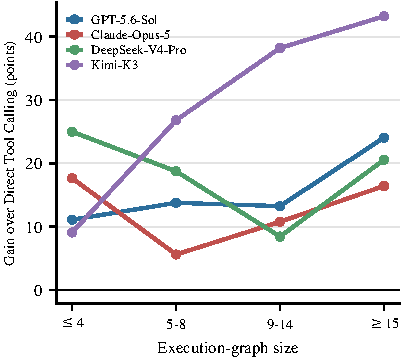
\includegraphics[width=\linewidth]{figs/scaling.pdf}\caption{Gain by execution-graph size}\label{fig:scaling}\end{subfigure}\hfill
\begin{subfigure}{0.32\linewidth}\centering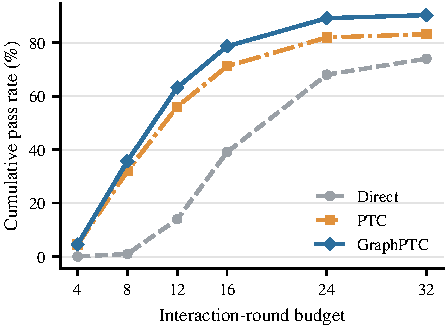
\includegraphics[width=\linewidth]{figs/efficiency.pdf}\caption{Accuracy vs. round budget}\label{fig:efficiency}\end{subfigure}\hfill
\begin{subfigure}{0.32\linewidth}\centering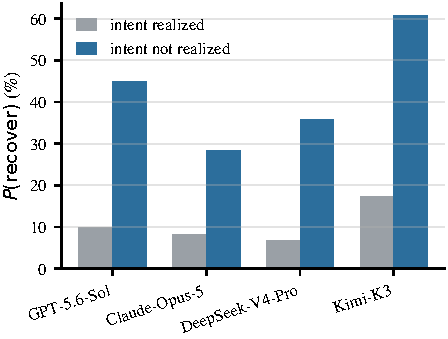
\includegraphics[width=\linewidth]{figs/recovery.pdf}\caption{Recovery probability by intent}\label{fig:recovery}\end{subfigure}
\caption{Analyses of GraphPTC on AppWorld, averaged over four backbones. (\subref{fig:scaling}) The gain over Direct Tool Calling is positive in every complexity bin, and its average widens toward the most complex tasks. (\subref{fig:efficiency}) Along the accuracy against interaction-round frontier GraphPTC reaches the accuracy of Direct Tool Calling with fewer rounds. (\subref{fig:recovery}) An intent that is not realized raises the probability that the agent issues a recovery action.}
\label{fig:analysis}
\end{figure}

\subsection{Ablation Study on Graph Modeling}

To locate the contribution of the graph layer, we ablate the two structural changes and report the five-backbone average of each setting.
Removing the execution graph and its graph-guided recovery reduces GraphPTC to PTC, where a block reports a plain success flag with raw output instead of typed effects, and removing the programmatic runtime as well reduces it to Direct Tool Calling.
As shown in Table~\ref{tab:ablation}, the execution graph is worth $6.3$ points on average and stays positive on all seven settings, while the programmatic runtime by itself is worth only $0.5$ points and turns negative on four of them, so writing code by itself does not reliably improve on Direct Tool Calling and the graph is what turns it into a consistent gain.

The size of the graph contribution tracks how much cross-block dependency a setting carries, reaching $11.7$ points on BrowseComp-Plus and $8.3$ points on AppWorld-Normal, where a result produced in one block is consumed by a later block, and falling to $1.9$ points on FRAMES, where most questions resolve within a few independent lookups.
The loss of plain PTC concentrates in the same settings and on one backbone, since its worst cells are $-33.0$ points on BrowseComp-Plus and $-34.5$ points on AppWorld-Normal, both on Claude-Opus-5, which loses $10.5$ points under plain PTC while the other four backbones gain from it.

\begin{table}[t]
\centering\scriptsize
\setlength{\abovecaptionskip}{0pt}
\setlength{\belowcaptionskip}{0pt}
\setlength{\tabcolsep}{4pt}
\newcommand{\hdc}[2]{\begin{tabular}[b]{@{}c@{}}\textbf{#1}\\\textbf{#2}\end{tabular}}
\caption{Ablation of the two structural changes of GraphPTC, reported per setting as the five-backbone average. PTC removes the execution graph and Direct Tool Calling removes the programmatic runtime as well, and the last two rows split the total gap into the contribution of each change.}
\label{tab:ablation}
\resizebox{\linewidth}{!}{%
\begin{tabular}{l ccccccc c}
\toprule
\textbf{Configuration}
 & \hdc{BrowseComp-}{Plus} & \hdc{AppWorld-}{Normal} & \hdc{AppWorld-}{Challenge} & \textbf{Agent-Diff} & \textbf{FanOutQA} & \textbf{FRAMES} & \hdc{Automation-}{Bench} & \textbf{Avg} \\
\midrule
\textbf{GraphPTC} (full)              & \best{39.1} & \best{92.1} & \best{88.4} & \best{72.7} & \best{63.7} & \best{81.0} & \best{31.7} & \best{67.0} \\
\;\; $-$ execution graph              & 27.4 & 83.8 & 83.7 & 67.3 & 55.2 & 79.1 & 27.8 & 60.6 \\
\;\; $-$ execution graph and programs & 33.1 & 82.4 & 69.3 & 69.7 & 61.2 & 79.4 & 26.0 & 60.2 \\
\midrule
Contribution of the execution graph     & $+11.7$ & $+8.3$ & $+4.7$ & $+5.4$ & $+8.5$ & $+1.9$ & $+3.9$ & $+6.3$ \\
Contribution of the programmatic runtime & $-5.7$ & $+1.4$ & $+14.4$ & $-2.4$ & $-6.0$ & $-0.4$ & $+1.8$ & $+0.5$ \\
\bottomrule
\end{tabular}%
}
\end{table}

\subsection{Advantage of Non-Linear Recovery}

To test whether modeling cross-block dependency as a graph enables recovery a linear history cannot, we study how the agent uses the actions that return to a specific node.
We measure the probability that the agent issues a recovery action conditioned on whether the previous block realized its declared intent, and on the tasks where GraphPTC uses recovery we compare its pass rate with PTC on the same task identifiers.
As shown in Figure~\ref{fig:recovery}, an unrealized intent raises the recovery probability by three to five times across backbones, so the declared-and-verified intent is an actionable signal that the agent responds to.
On the same task identifiers GraphPTC exceeds PTC, and since the comparison fixes the task and differs mainly in whether the agent can return to a failed node, we read the gap as largely driven by non-linear recovery.

\subsection{Advantage on Complex Long-Horizon Tasks}

To locate where the advantage of GraphPTC arises, we bin every AppWorld task by the number of program blocks in its execution graph and measure the gain of GraphPTC over Direct Tool Calling within each bin.
As shown in Figure~\ref{fig:scaling}, the gain is positive in every bin for every backbone, and its four-backbone average rises from $15.7$ points in the smallest bin to $26.1$ points in the largest.
The widening is carried by GPT-5.6-Sol and Kimi-K3, which reach $24.1$ and $43.2$ points in the largest bin, while Claude-Opus-5 and DeepSeek-V4-Pro gain in every bin without a monotone trend.
A larger task graph holds more intermediate results and more failure-prone steps, so addressable artifacts and local recovery matter more as a linear history grows harder to reconstruct.

\subsection{Efficiency and Token Economy}

To check whether the graph improves efficiency and not only accuracy, we measure the interaction rounds each method spends and trace the accuracy it reaches under a round budget.
On AutomationBench, GraphPTC spends $54$ to $64\%$ fewer model rounds than Direct Tool Calling while raising the pass rate, because one block carries several dependent calls whose intermediate values are registered as artifacts and reused (Appendix~\ref{app:analyses}).
As shown in Figure~\ref{fig:efficiency}, on AppWorld the same effect appears along the accuracy against round frontier, where GraphPTC reaches the accuracy of Direct Tool Calling with about $2$ times fewer rounds and stays on or above the PTC frontier at every budget.
The graph stays in the runtime and enters the model only through the bounded feedback, so the input per round is independent of graph size and the round savings are not offset by a growing context.
As shown in Table~\ref{tab:cost}, GraphPTC reaches higher accuracy than Direct Tool Calling on every benchmark while reading $1.7$ to $2.3$ times fewer input tokens, and uses fewer rounds on all but one benchmark, since a per-call transcript re-sends the growing history on each turn.

\begin{table}[t]
\centering\scriptsize
\setlength{\abovecaptionskip}{0pt}
\setlength{\belowcaptionskip}{0pt}
\setlength{\tabcolsep}{5pt}
\caption{Cost comparison of GraphPTC and Direct Tool Calling, averaged over four backbones. GraphPTC reaches higher accuracy while reading fewer input tokens on every benchmark and using fewer interaction rounds on all but one. \textbf{Bold} marks the better method per metric and benchmark.}
\label{tab:cost}
\resizebox{\linewidth}{!}{%
\begin{tabular}{l cc cc cc}
\toprule
 & \multicolumn{2}{c}{\textbf{Accuracy (\%)}} & \multicolumn{2}{c}{\textbf{Input tokens (k)}} & \multicolumn{2}{c}{\textbf{Rounds}} \\
\cmidrule(lr){2-3}\cmidrule(lr){4-5}\cmidrule(lr){6-7}
\textbf{Benchmark} & Direct Tool Calling & GraphPTC & Direct Tool Calling & GraphPTC & Direct Tool Calling & GraphPTC \\
\midrule
AppWorld-Normal    & 82.3 & \best{90.9} & 151.4 & \best{84.1}  & 16.4 & \best{9.1} \\
AppWorld-Challenge & 68.7 & \best{88.6} & 228.8 & \best{133.5} & 18.7 & \best{11.7} \\
Agent-Diff         & 68.5 & \best{70.8} & 113.2 & \best{49.0}  & 9.6  & \best{6.6} \\
FanOutQA           & 60.0 & \best{62.9} & 128.5 & \best{63.9}  & 8.7  & \best{6.9} \\
FRAMES             & 79.3 & \best{80.6} & 93.0  & \best{55.2}  & \best{5.6}  & 7.1 \\
AutomationBench    & 24.6 & \best{29.0} & 324.4 & \best{171.9} & 36.1 & \best{14.3} \\
\bottomrule
\end{tabular}%
}
\end{table}

\begin{figure}[t]
\centering
\begin{subfigure}{0.32\linewidth}\centering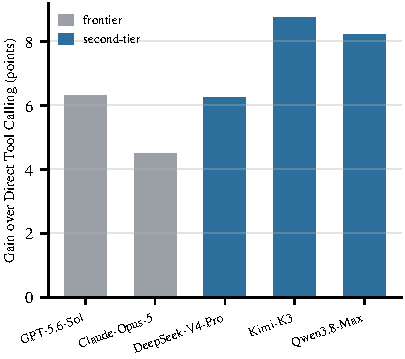
\includegraphics[width=\linewidth]{figs/gain.pdf}\caption{Gain over Direct by backbone}\label{fig:capgain}\end{subfigure}\hfill
\begin{subfigure}{0.32\linewidth}\centering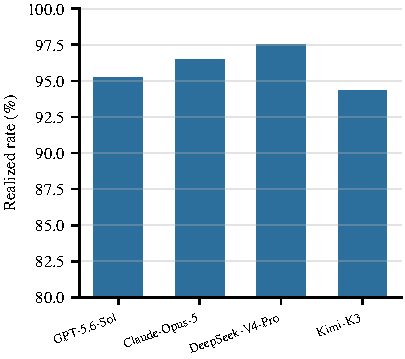
\includegraphics[width=\linewidth]{figs/fidelity.pdf}\caption{Realization rate of intents}\label{fig:fidelity}\end{subfigure}\hfill
\begin{subfigure}{0.32\linewidth}\centering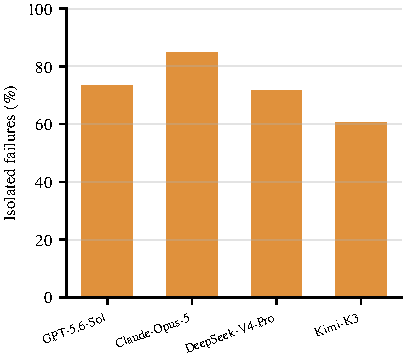
\includegraphics[width=\linewidth]{figs/isolation.pdf}\caption{Isolation rate of failures}\label{fig:isolation}\end{subfigure}
\caption{Further analyses of GraphPTC. (\subref{fig:capgain}) Gain over Direct Tool Calling by backbone on the seven-setting average; the second-tier backbones gain more from the graph than the frontier ones. (\subref{fig:fidelity}) On AppWorld over four backbones, most declared expected changes are realized in the graph. (\subref{fig:isolation}) On AppWorld over four backbones, most block failures are isolated, with no further failure within three blocks.}
\label{fig:analysis2}
\end{figure}

\subsection{Robustness across Backbone Capability}

To examine how the benefit depends on backbone capability, we group the five backbones into frontier ones, GPT-5.6-Sol and Claude-Opus-5, and second-tier ones, DeepSeek-V4-Pro, Kimi-K3, and Qwen3.8-Max, and compare the gain over Direct Tool Calling.
As shown in Figure~\ref{fig:capgain}, the second-tier backbones gain more than the frontier ones.
This follows because the execution graph externalizes the state tracking and dependency bookkeeping that a frontier model partly carries on its own, so a second-tier model benefits more when that structure is supplied.
At the same time, the graph is what keeps PTC from collapsing on a frontier backbone, since Claude-Opus-5 loses accuracy under plain PTC yet reaches the best result under GraphPTC.

\subsection{Reliability of the Intent Signal}

To assess whether the progress signal the agent acts on is trustworthy, we measure how often a declared expected change is realized in the graph and how often a block failure stays local.
As shown in Figure~\ref{fig:fidelity}, the declared intent is realized in more than nine of ten blocks across backbones, so the signal that drives recovery is grounded in observed effects and not in self-report.
As shown in Figure~\ref{fig:isolation}, most block failures under GraphPTC are isolated with no further failure in the next three blocks, while under plain PTC a failing task tends to repeat the same exception.

\subsection{Limitations}

Our study is inference-time and adds no training, so a backbone that cannot follow the intent declaration gains less from the graph.
We report one run per setting and treat the agreement of the trend across five backbones and seven settings as the evidence of robustness.
The controlled comparison holds tools, prompts, and budgets fixed, so it isolates the graph but does not combine GraphPTC with reflection or long-term memory, which could be layered on the same graph.

\section{Conclusion}

In this paper, we propose \method, which models programmatic tool calling as a task-level dynamic execution graph.
Specifically, \method turns the linear execution history of PTC into a typed structure over in-block tool effects and cross-block dependencies, so the agent reads what an execution changed and chooses to continue, patch, replan, or answer.
Across seven benchmark settings and five backbones, \method is the best method in every case, improving over PTC by $6.3$ points and over Direct Tool Calling by $6.8$ points while reading $1.7$ to $2.3$ times fewer input tokens.
Indexing what an execution did and not only what an agent saw is a broadly useful design pattern for agents that act on their own history.


\subsection*{Reproducibility Statement}
The method is specified in Section~\ref{sec:method} and Algorithm~\ref{alg:graphptc}, with node and edge types in Appendix~\ref{app:types} and further details in Appendix~\ref{app:impl}. All arms share one protocol described in Section~\ref{sec:experiments-setup}, and the plotting code and the raw numbers behind every analysis figure are released under the \texttt{code/} directory.

\subsection*{AI Use Statement}
Generative AI tools were used to assist with language editing of the manuscript. All technical content, experiments, and analyses were designed, run, and verified by the authors, who take responsibility for the final content.

\bibliography{graphptc}
\bibliographystyle{iclr2027_conference}

\appendix
\section{Node and Edge Types of the Execution Graph}
\label{app:types}

Table~\ref{tab:types} lists the typed nodes and edges maintained in the execution graph.
Node types cover the task, program blocks, tool or API calls with read or write effects, artifacts, state versions and state effects, failures, and action intents.
Edge types cover execution structure, data flow, state evolution, failure attribution, cross-block equivalence and reuse, and intent binding.

\begin{table}[h]
\centering\small
\setlength{\tabcolsep}{6pt}
\begin{tabular}{ll}
\toprule
\textbf{Category} & \textbf{Types} \\
\midrule
Nodes & \texttt{TASK}, \texttt{BLOCK}, \texttt{CALL} (\texttt{read}/\texttt{write}), \texttt{ARTIFACT}, \texttt{STATE}, \texttt{FAILURE}, \texttt{INTENT} \\
Execution & \texttt{contains}, \texttt{executes}, \texttt{produces}, \texttt{fails\_at} \\
Data flow & \texttt{consumes}, \texttt{reuses}, \texttt{derives} \\
State & \texttt{reads}, \texttt{writes}, \texttt{mutates}, \texttt{supersedes} \\
Cross-block & \texttt{equivalent\_to} \\
Intent & \texttt{targets}, \texttt{implemented\_by} \\
\bottomrule
\end{tabular}
\caption{Node and edge types of the dynamic execution graph.}
\label{tab:types}
\end{table}

\section{Implementation Details}
\label{app:impl}

The execution graph is maintained incrementally with node and edge cursors, so extracting the round delta $\Delta_t$ visits only the nodes and edges added in the current round and does not solve a general graph edit distance.
Tool wrappers record arguments, results, and effects during execution, and the trace projector attaches these to the current block after execution.
Cross-block equivalence uses tool effect contracts to normalize argument and result identities, so cached deterministic reads may be reused while tools with side effects follow their contract.
The bounded feedback prunes list items first and then reduces fields under the character budget $B$, and the full graph is retained at runtime and never sent to the model in whole.

\section{Additional Analyses}
\label{app:analyses}

\textbf{Scenario Goal Completion on AppWorld.}\quad
Table~\ref{tab:sgc} reports the secondary AppWorld metric, Scenario Goal Completion, which requires every task in a scenario to succeed together.
GraphPTC improves Scenario Goal Completion on both splits for every backbone, and the margin over PTC is wider than on Task Goal Completion, which matches the intuition that a scenario is only as strong as its most dependent step.

\begin{table}[h]
\centering\scriptsize
\setlength{\tabcolsep}{6pt}
\begin{tabular}{l cc cc}
\toprule
 & \multicolumn{2}{c}{\textbf{AppWorld-Normal}} & \multicolumn{2}{c}{\textbf{AppWorld-Challenge}} \\
\cmidrule(lr){2-3}\cmidrule(lr){4-5}
\textbf{Backbone} & \textbf{PTC} & \textbf{GraphPTC} & \textbf{PTC} & \textbf{GraphPTC} \\
\midrule
GPT-5.6-Sol     & 83.90 & \best{85.70} & 82.00 & \best{87.10} \\
Claude-Opus-5   & 46.40 & \best{92.90} & 69.10 & \best{92.10} \\
DeepSeek-V4-Pro & 80.40 & \best{82.10} & 66.90 & \best{88.50} \\
Kimi-K3         & 67.90 & \best{76.80} & 66.90 & \best{70.50} \\
\bottomrule
\end{tabular}
\caption{Scenario Goal Completion on AppWorld. \textbf{Bold} marks the better method per backbone and split. GraphPTC improves the scenario metric on every backbone and split.}
\label{tab:sgc}
\end{table}

\textbf{Use of the recovery actions.}\quad
Table~\ref{tab:actions} counts how often the agent issues \textsc{Patch} and \textsc{Replan} on AppWorld and the pass rate of the tasks that use them.
The recovery actions are used on a large share of tasks, and the tasks that trigger a \textsc{Patch} still pass in almost all cases, which shows the graph turns a failure into a targeted retry that usually succeeds.

\begin{table}[h]
\centering\scriptsize
\setlength{\tabcolsep}{6pt}
\begin{tabular}{l ccc}
\toprule
\textbf{Backbone} & \textbf{\textsc{Patch} calls} & \textbf{\textsc{Replan} calls} & \textbf{Pass rate on \textsc{Patch} tasks} \\
\midrule
GPT-5.6-Sol     & 516 & 52 & 100.0 \\
Claude-Opus-5   & 506 & 20 & 97.8 \\
DeepSeek-V4-Pro & 586 & 0  & 94.7 \\
Kimi-K3         & 972 & 3  & 99.1 \\
\bottomrule
\end{tabular}
\caption{Use of the recovery actions on AppWorld, summed over the normal and challenge splits. Tasks that trigger a \textsc{Patch} pass in almost all cases.}
\label{tab:actions}
\end{table}

\textbf{Interaction rounds on AutomationBench.}\quad
Table~\ref{tab:ab-rounds} reports the average model rounds per task on AutomationBench.
GraphPTC spends $54$ to $64\%$ fewer rounds than Direct Tool Calling on every backbone while reaching a higher completion rate, which complements the AppWorld frontier in the main text and shows the efficiency gain is not specific to one benchmark.

\begin{table}[h]
\centering\scriptsize
\setlength{\tabcolsep}{6pt}
\begin{tabular}{l ccc}
\toprule
\textbf{Backbone} & \textbf{Direct Tool Calling} & \textbf{GraphPTC} & \textbf{Fewer rounds} \\
\midrule
GPT-5.6-Sol     & 32.4 & 11.5 & 64\% \\
Claude-Opus-5   & 27.0 & 11.6 & 57\% \\
DeepSeek-V4-Pro & 54.8 & 20.1 & 63\% \\
Kimi-K3         & 30.2 & 13.9 & 54\% \\
\bottomrule
\end{tabular}
\caption{Average model rounds per task on AutomationBench. GraphPTC reaches a higher completion rate with far fewer rounds on every backbone.}
\label{tab:ab-rounds}
\end{table}

\textbf{Input tokens across benchmarks.}\quad
Table~\ref{tab:tokens-multi} reports the mean input tokens a task consumes, averaged over the four backbones, for six benchmarks.
On every benchmark GraphPTC reads far fewer input tokens than Direct Tool Calling and only modestly more than PTC, so the token economy shown for AppWorld in the main text holds throughout, since a per-call transcript re-sends the growing history on each turn while the bounded feedback does not.

\begin{table}[h]
\centering\scriptsize
\setlength{\tabcolsep}{6pt}
\begin{tabular}{l ccc}
\toprule
\textbf{Benchmark} & \textbf{Direct Tool Calling} & \textbf{PTC} & \textbf{GraphPTC} \\
\midrule
AppWorld-Normal    & 151.4k & 60.2k  & 84.1k \\
AppWorld-Challenge & 228.8k & 97.3k  & 133.5k \\
Agent-Diff         & 113.2k & 34.4k  & 49.0k \\
FanOutQA           & 128.5k & 49.5k  & 63.9k \\
FRAMES             & 93.0k  & 42.2k  & 55.2k \\
AutomationBench    & 324.4k & 156.6k & 171.9k \\
\bottomrule
\end{tabular}
\caption{Mean input tokens per task, averaged over the four backbones. GraphPTC reads far fewer input tokens than Direct Tool Calling on every benchmark while reaching the best accuracy.}
\label{tab:tokens-multi}
\end{table}

\textbf{Gain by reasoning type on FRAMES.}\quad
Table~\ref{tab:frames-type} breaks the FRAMES gain down by reasoning type for the two closed backbones.
The gain is largest on post-processing and temporal reasoning, where an answer must combine results across several calls, which is where cross-block linking removes the most redundant work.

\begin{table}[h]
\centering\scriptsize
\setlength{\tabcolsep}{6pt}
\begin{tabular}{l ccccc}
\toprule
\textbf{Backbone} & \begin{tabular}[b]{@{}c@{}}Multiple\\constraints\end{tabular} & \begin{tabular}[b]{@{}c@{}}Numerical\end{tabular} & \begin{tabular}[b]{@{}c@{}}Post-\\processing\end{tabular} & \begin{tabular}[b]{@{}c@{}}Tabular\end{tabular} & \begin{tabular}[b]{@{}c@{}}Temporal\end{tabular} \\
\midrule
GPT-5.6-Sol   & +1.5 & +1.4 & +4.7 & +1.7 & +2.2 \\
Claude-Opus-5 & $-0.6$ & +1.4 & +0.9 & +0.4 & +2.2 \\
\bottomrule
\end{tabular}
\caption{FRAMES gain of GraphPTC over the stronger baseline by reasoning type, in accuracy points. The gain concentrates on post-processing and temporal reasoning.}
\label{tab:frames-type}
\end{table}

\textbf{Where the workflow gain arises.}\quad
Agent-Diff labels each task by the operations it performs, and Table~\ref{tab:opsplit} splits the tasks by whether they update or delete existing state.
GraphPTC improves over PTC by $7.2$ points on the state-overwriting tasks and by essentially nothing on the tasks with no overwrite, which matches the mechanism, since the state versioning of the graph helps exactly where a later step depends on a mutated state and adds little where there is no state to track.

\begin{table}[h]
\centering\scriptsize
\setlength{\tabcolsep}{6pt}
\begin{tabular}{l cccc}
\toprule
\textbf{Task type} & \textbf{\#tasks} & \textbf{Direct Tool Calling} & \textbf{PTC} & \textbf{GraphPTC} \\
\midrule
Update or delete state & 1649 & 63.3 & 58.3 & \best{65.5} \\
No state overwrite      & 654  & \best{79.2} & 79.0 & 78.7 \\
\bottomrule
\end{tabular}
\caption{Agent-Diff pass rate split by whether a task overwrites existing state, aggregated over the four backbones. GraphPTC's gain concentrates on state-overwriting tasks, where the state versioning of the graph applies.}
\label{tab:opsplit}
\end{table}

\section{Case Studies}
\label{app:cases}

Figure~\ref{fig:casegraph} draws an example execution graph and marks the three mechanisms discussed below. Each trace is abbreviated to the relevant blocks.

\begin{figure}[t]
\centering
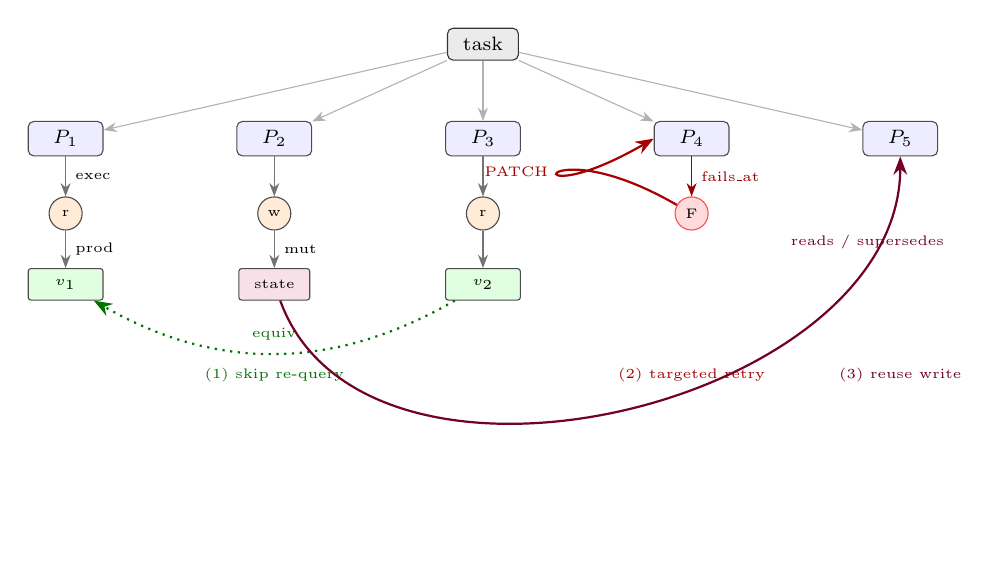
\begin{tikzpicture}[
  font=\scriptsize,
  blk/.style={rounded corners=2pt, draw=black!70, fill=blue!7, minimum width=0.95cm, minimum height=0.42cm, align=center},
  tsk/.style={rounded corners=2pt, draw=black!80, fill=black!8, minimum width=0.9cm, minimum height=0.4cm, align=center},
  call/.style={circle, draw=black!70, fill=orange!16, minimum size=0.42cm, inner sep=0.5pt, align=center},
  art/.style={rounded corners=1pt, draw=black!70, fill=green!12, minimum width=0.95cm, minimum height=0.4cm, align=center},
  st/.style={rounded corners=1pt, draw=black!70, fill=purple!12, minimum width=0.9cm, minimum height=0.4cm, align=center},
  fail/.style={circle, draw=red!70, fill=red!14, minimum size=0.42cm, inner sep=0.5pt, align=center},
  rel/.style={->, >=Stealth, draw=black!55, thin},
  faint/.style={->, >=Stealth, draw=black!30, thin},
]
% task
\node[tsk] (t) at (5.3,3.3) {task};
% blocks
\node[blk] (b1) at (0,2.1) {$P_1$};
\node[blk] (b2) at (2.65,2.1) {$P_2$};
\node[blk] (b3) at (5.3,2.1) {$P_3$};
\node[blk] (b4) at (7.95,2.1) {$P_4$};
\node[blk] (b5) at (10.6,2.1) {$P_5$};
\foreach \b in {b1,b2,b3,b4,b5}{\draw[faint] (t)--(\b);}

% B1: read -> artifact a1
\node[call] (c1) at (0,1.15) {\tiny r};
\node[art]  (a1) at (0,0.25) {\tiny $v_1$};
\draw[rel] (b1)--(c1) node[midway,right,font=\tiny]{exec};
\draw[rel] (c1)--(a1) node[midway,right,font=\tiny]{prod};

% B2: write -> state s1
\node[call] (c2) at (2.65,1.15) {\tiny w};
\node[st]   (s1) at (2.65,0.25) {\tiny state};
\draw[rel] (b2)--(c2);
\draw[rel] (c2)--(s1) node[midway,right,font=\tiny]{mut};

% B3: read -> artifact a2, equiv to a1  (Case 1)
\node[call] (c3) at (5.3,1.15) {\tiny r};
\node[art]  (a2) at (5.3,0.25) {\tiny $v_2$};
\draw[rel] (b3)--(c3);
\draw[rel] (c3)--(a2);
\draw[->, >=Stealth, dotted, green!45!black, thick] (a2) to[out=210,in=-30] node[midway,above=1pt,font=\tiny,text=green!45!black]{equiv} (a1);
\node[font=\tiny, text=green!45!black] at (2.65,-0.9) {(1) skip re-query};

% B4: failure + PATCH  (Case 2)
\node[fail] (f) at (7.95,1.15) {\tiny F};
\draw[rel,red!60!black] (b4)--(f) node[midway,right,font=\tiny,text=red!60!black]{fails\_at};
\draw[->, >=Stealth, red!65!black, thick] (f) to[out=150,in=210,looseness=6] node[midway,left,font=\tiny,text=red!65!black]{PATCH} (b4.west);
\node[font=\tiny, text=red!65!black] at (7.95,-0.9) {(2) targeted retry};

% B5: reads earlier state via supersedes  (Case 3)
\draw[->, >=Stealth, purple!60!black, thick] (s1) to[out=-70,in=-90] node[pos=0.85,above,font=\tiny,text=purple!60!black]{reads / supersedes} (b5);
\node[font=\tiny, text=purple!60!black] at (10.6,-0.9) {(3) reuse write};

\end{tikzpicture}
\caption{An example execution graph built by GraphPTC. Blocks $P_t$ are projected into typed calls (read $r$, write $w$), artifacts $v$, states, and failures $F$. (1) block $P_3$ produces $v_2$ that an \texttt{equivalent\_to} edge links to the earlier $v_1$, so the agent skips a redundant query. (2) a failed call in $P_4$ adds a \texttt{FAILURE} the agent repairs with a targeted \textsc{Patch} instead of re-running the block. (3) block $P_5$ reads the state written by $P_2$ through the \texttt{supersedes} chain instead of re-deriving it.}
\label{fig:casegraph}
\end{figure}


\textbf{Case 1: cross-block equivalence removes redundant retrieval.}\quad
On a multi-hop question, block $P_1$ queries \emph{population of the capital of country X} and block $P_3$ later queries \emph{capital city X population}.
The trace projector assigns both results the same identity key and adds an \texttt{equivalent\_to} edge (mark (1) in Figure~\ref{fig:casegraph}), and the feedback reports the second result as equivalent.
Under PTC the same content returns as a fresh output string, and the agent issues a third query to reconcile them, whereas under GraphPTC the agent reads the existing artifact and moves to the next hop.

\textbf{Case 2: a failed write becomes a targeted patch.}\quad
On an AppWorld task, block $P_4$ posts a payment whose call raises an error, so the projector adds a \texttt{FAILURE} node with a \texttt{fails\_at} edge and the feedback marks the intent unrealized (mark (2)).
The agent declares \textsc{Patch} on the same target, fixes the malformed field, and re-executes only that step.
Under PTC the failure is one line inside a long output, and the agent re-runs the whole block, which re-issues the calls that had already succeeded.

\textbf{Case 3: a later block links to an earlier write instead of re-deriving it.}\quad
On a workflow task, block $P_2$ updates a contact record and block $P_5$ needs the updated field.
The state is versioned with a \texttt{supersedes} edge, so the feedback points block $P_5$ at the current version and the agent reads it directly (mark (3)).
Under PTC the agent re-fetches the record to be sure of its value, which adds a round and risks reading a stale copy from earlier in the transcript.


\end{document}
